\section{结果与讨论}

% Wide figures are declared before the running text so the compositor can fill each page.

\begin{figure*}[!tbp]
\begin{minipage}{\textwidth}
\centering
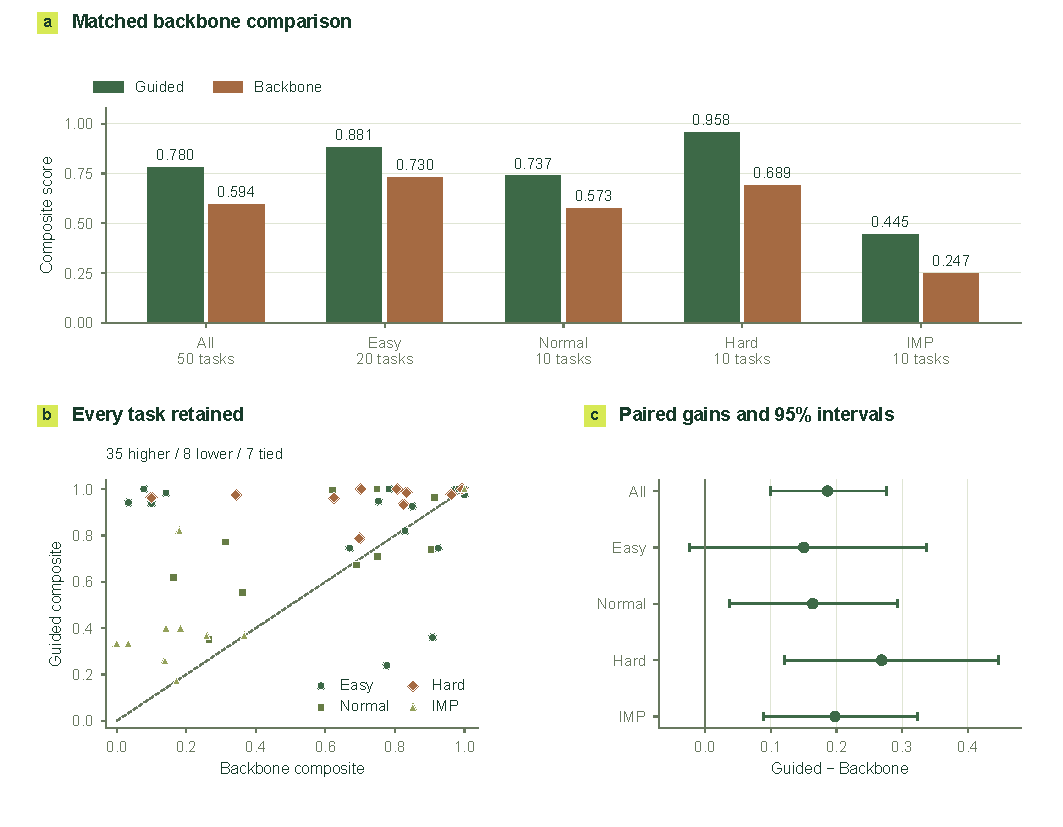
\includegraphics[width=\textwidth]{figures/bench_overview.pdf}
\caption{P2 主比较与逐题差异。a，Cloudra Guided 与同一 backbone 的 Standard 基线在全部 50 题及各难度层的整理后复合分；Easy 为 20 题，其余各 10 题。b，保留全部 50 个同题配对。c，配对均差与 100,000 次按任务整组 bootstrap 的 95\% 百分位区间。}
\label{fig:bench-overview}
\end{minipage}
\end{figure*}

\begin{figure*}[!tbp]
\begin{minipage}{\textwidth}
\centering
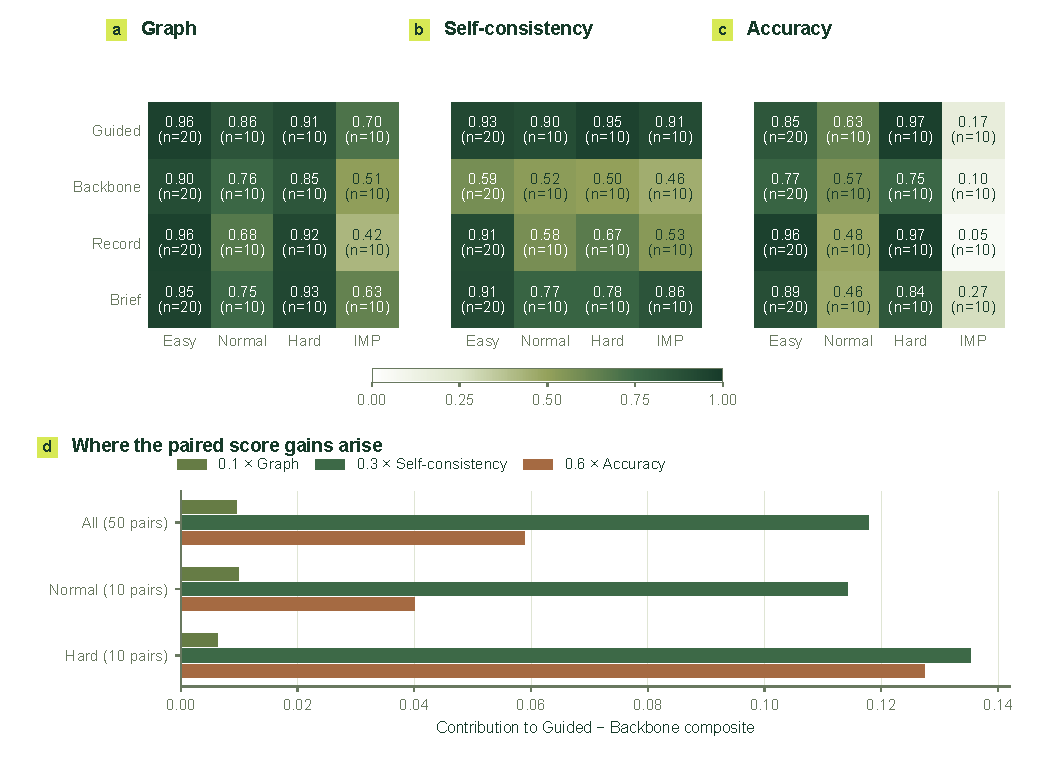
\includegraphics[width=\textwidth]{figures/bench_components.pdf}
\caption{全部200次整理后运行的三个评分层。a--c，各配置、难度层的Graph、自洽性与Accuracy均值；每配置总体50题，Easy为20题，其余各层10题。d，按固定0.1/0.3/0.6权重分解Guided相对Backbone的均差，全部、Normal与Hard分别使用完整50、10和10个配对。各运行分量由其自身研究材料与评分记录对齐至最终整理总分。}
\label{fig:bench-components}
\end{minipage}
\end{figure*}

\begin{figure*}[!tbp]
\begin{minipage}{\textwidth}
\centering
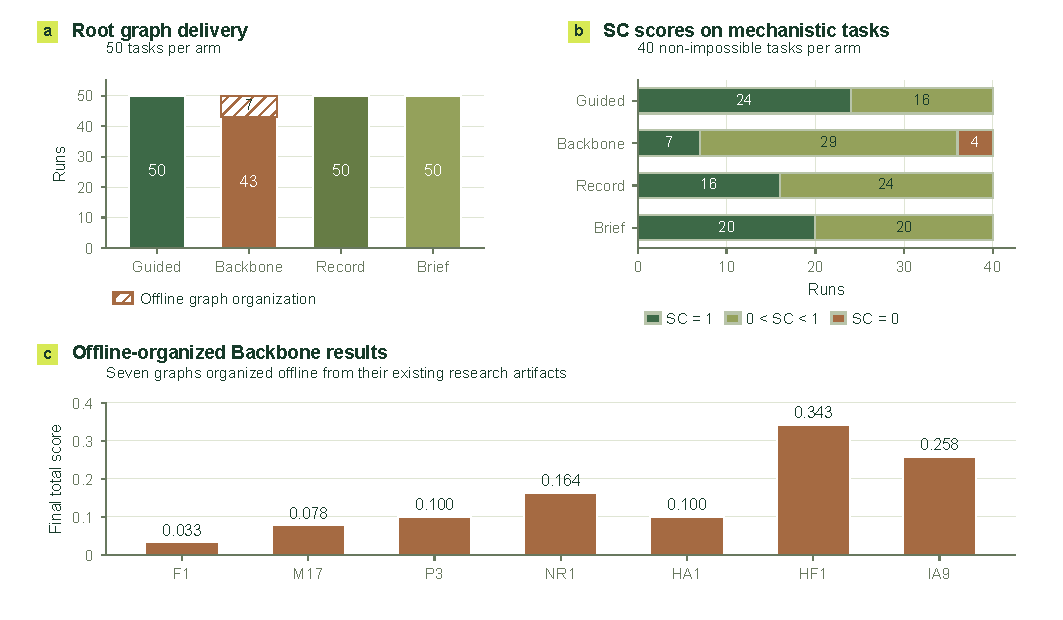
\includegraphics[width=\textwidth]{figures/bench_delivery.pdf}
\caption{运行期交付图与最终科学支持。a，每配置50题中的原始根图记录，Guided、Backbone、Record与Brief分别为50、43、50和50；斜线标记从运行自身材料离线组装的7份Backbone图，整理后每配置均为50份。b，每配置全部40道非Impossible题的自洽分布，区分SC=1、部分正分及SC=0；满分数依次为24、7、16和20，Backbone另有4题零分。c，7个未在运行中形成根图的Backbone任务整理后总分，范围0.0333至0.3425，均值0.1537。}
\label{fig:bench-delivery}
\end{minipage}
\end{figure*}

\begin{figure*}[!tbp]
\begin{minipage}{\textwidth}
\centering
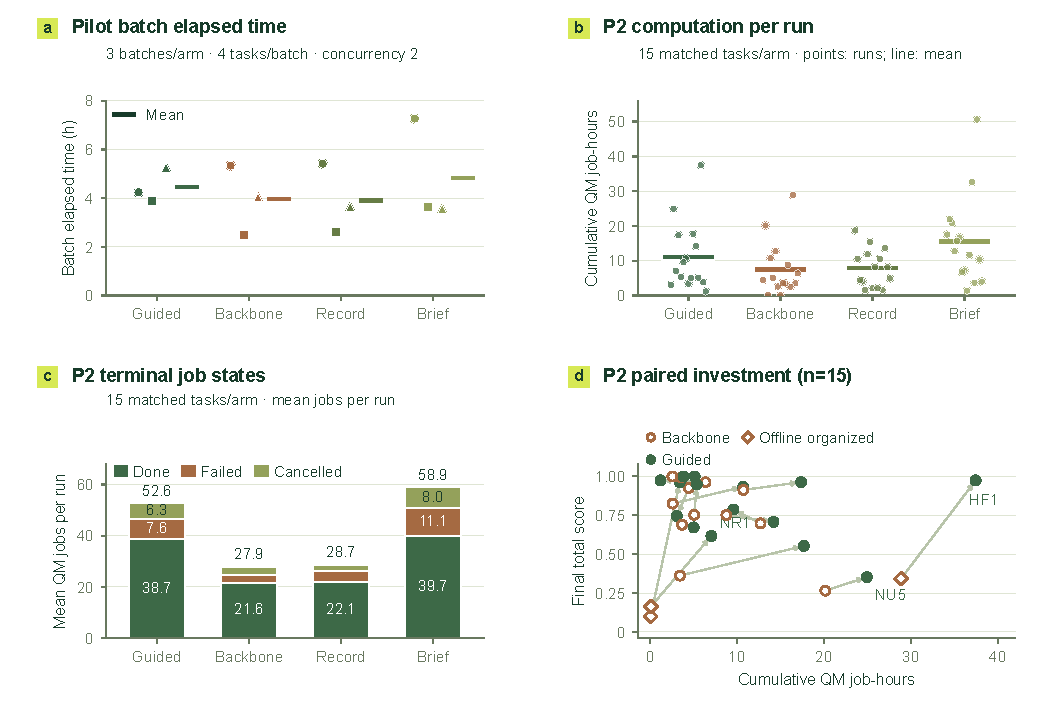
\includegraphics[width=\textwidth]{figures/bench_speed.pdf}
\caption{运行速度与计算投入。a，P1b 的 12 个真实批次，每配置 3 批，每批 4 题，并发为 2；点为观测批次，短线为均值。b，P2 四配置共同 15 题的逐运行累计 QM job-hours 及均值。c，同一任务集每运行的完成、失败和取消作业数量。d，Standard 与 Guided 同题的计算投入及整理后总分，箭头连接相同任务，菱形标记离线组装机理图的运行。}
\label{fig:bench-speed}
\end{minipage}
\end{figure*}

\begin{figure*}[p]
\begin{minipage}{\textwidth}
\centering
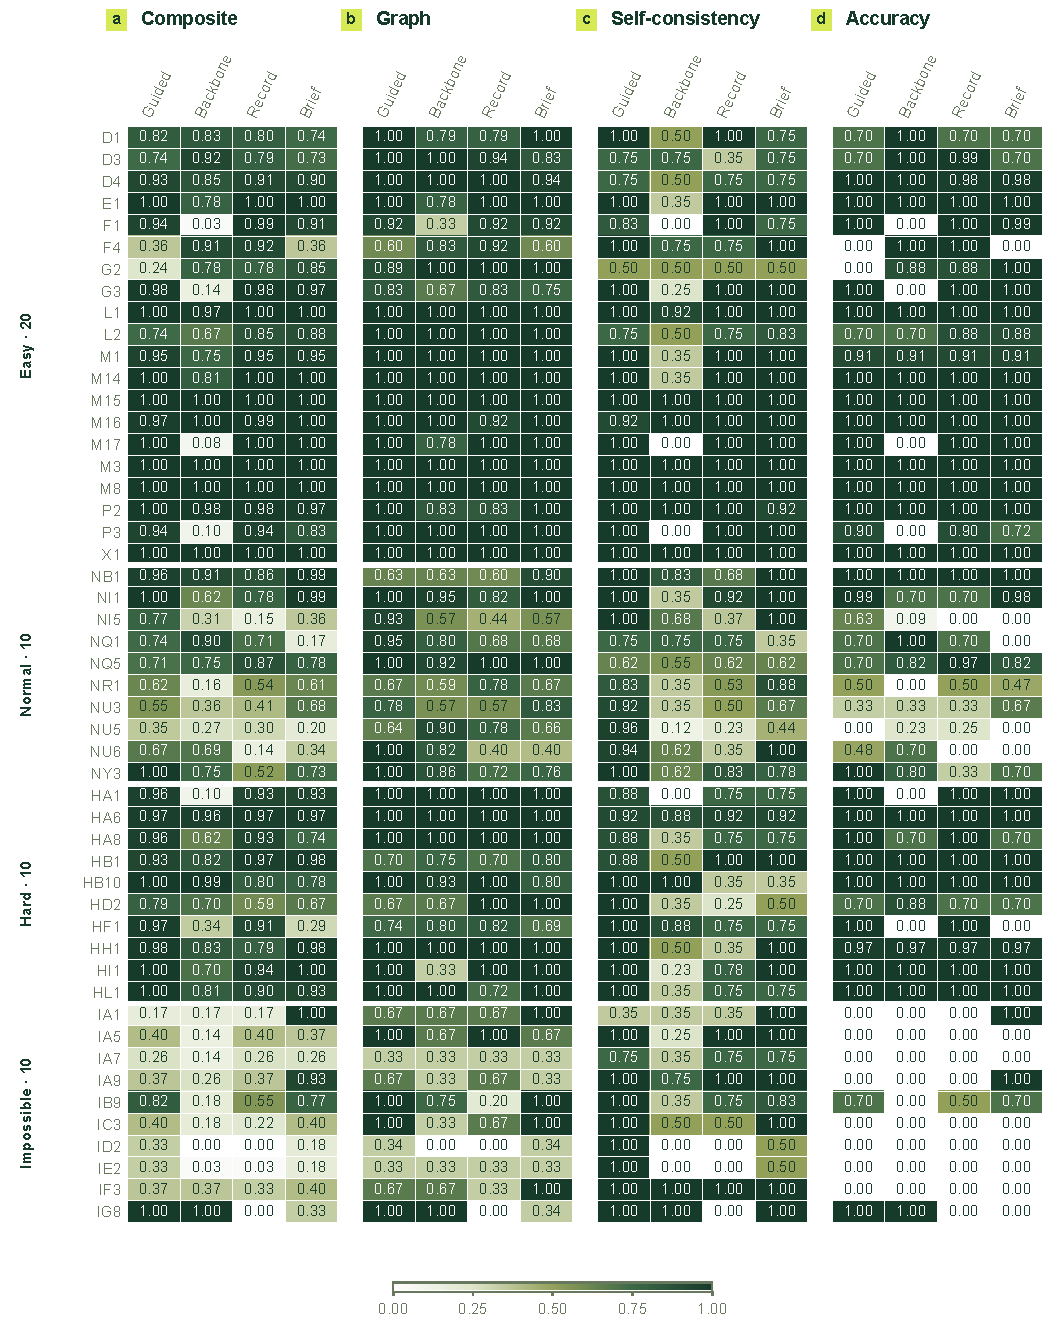
\includegraphics[width=\textwidth]{figures/bench_tasks_all.pdf}
\caption{CloudraBench全部50题、四配置的完整逐题成绩。四个评分块按相同顺序展示综合分、Graph、自洽性与Accuracy，色标统一为0--1，800格全部呈现。数值保留两位小数，来源表保留完整精度。}
\label{fig:bench-tasks}
\vspace{6pt}
\end{minipage}
\end{figure*}

\begin{figure*}[!tbp]
\begin{minipage}{\textwidth}
\centering
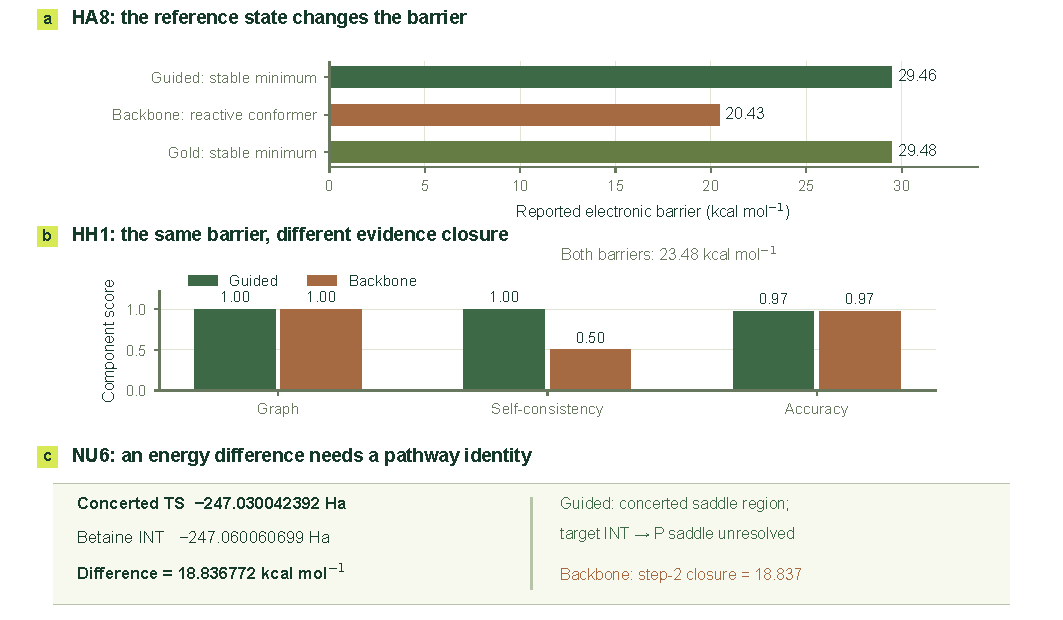
\includegraphics[width=\textwidth]{figures/bench_cases.pdf}
\caption{计算结果的科学归属。a，HA8 分别采用稳定极小值与反应性构象作参照的声明能垒，与 campaign Gold 并列。b，HH1 两组均给出 23.48 kcal/mol 能垒且准确度接近，自洽证据分不同。c，NU6 两个已记录能量之差为 18.836772 kcal/mol；Guided 将其保留为 concerted 鞍点区域的代价，并将目标闭环鞍点留为未解决，Standard 则将 18.837 声明为第二步闭环能垒。计算细节与路径文字取自归档证据记录。}
\label{fig:bench-cases}
\end{minipage}
\end{figure*}

\begin{figure*}[!tbp]
\begin{minipage}{\textwidth}
\centering
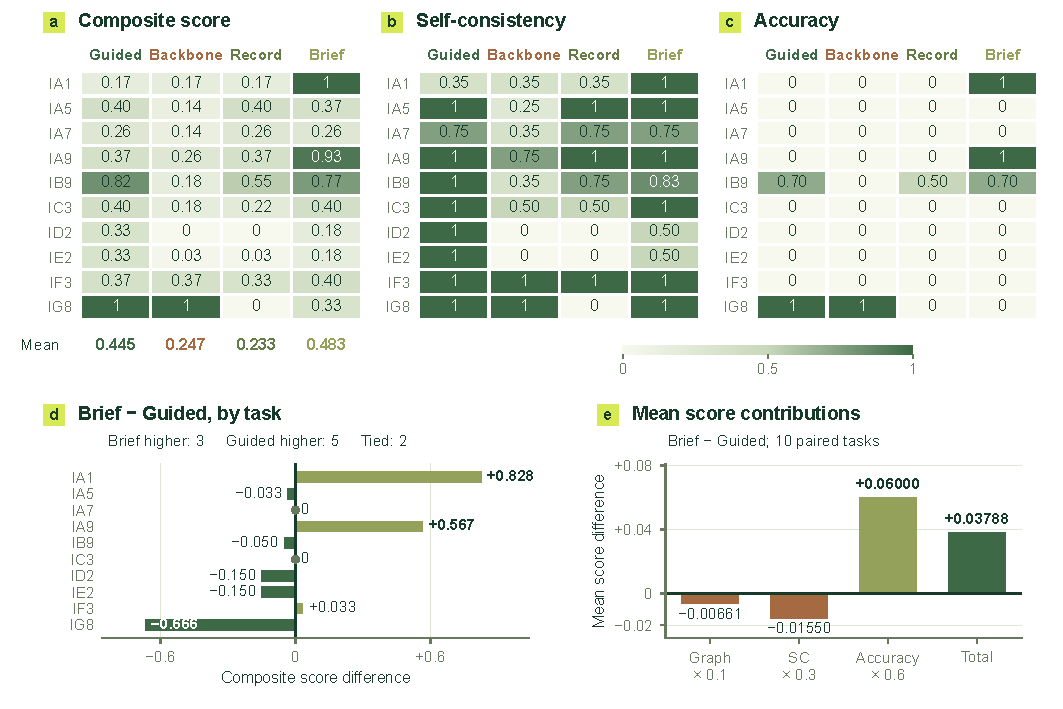
\includegraphics[width=\textwidth]{figures/bench_imp.pdf}
\caption{Impossible层的逐题对照与Brief--Guided差异。a--c，全部10题、四配置的完整整理总分、自洽性和Accuracy，色标统一为0--1。d，Brief相对Guided的逐题总分差，均差+0.03788集中于IA1与IA9，IG8呈相反结果；Guided赢5题、Brief赢3题、2题持平。e，按既定权重分解均差，Accuracy贡献+0.06000、Graph贡献$-0.00661$、自洽性贡献$-0.01550$，细微加总差异来自保存总分的舍入；任务bootstrap的95\%区间为$-0.188$至+0.284，逐题科学声明见下文分析。}
\label{fig:bench-imp}
\end{minipage}
\end{figure*}

\begin{figure*}[!tbp]
\begin{minipage}{\textwidth}

\centering
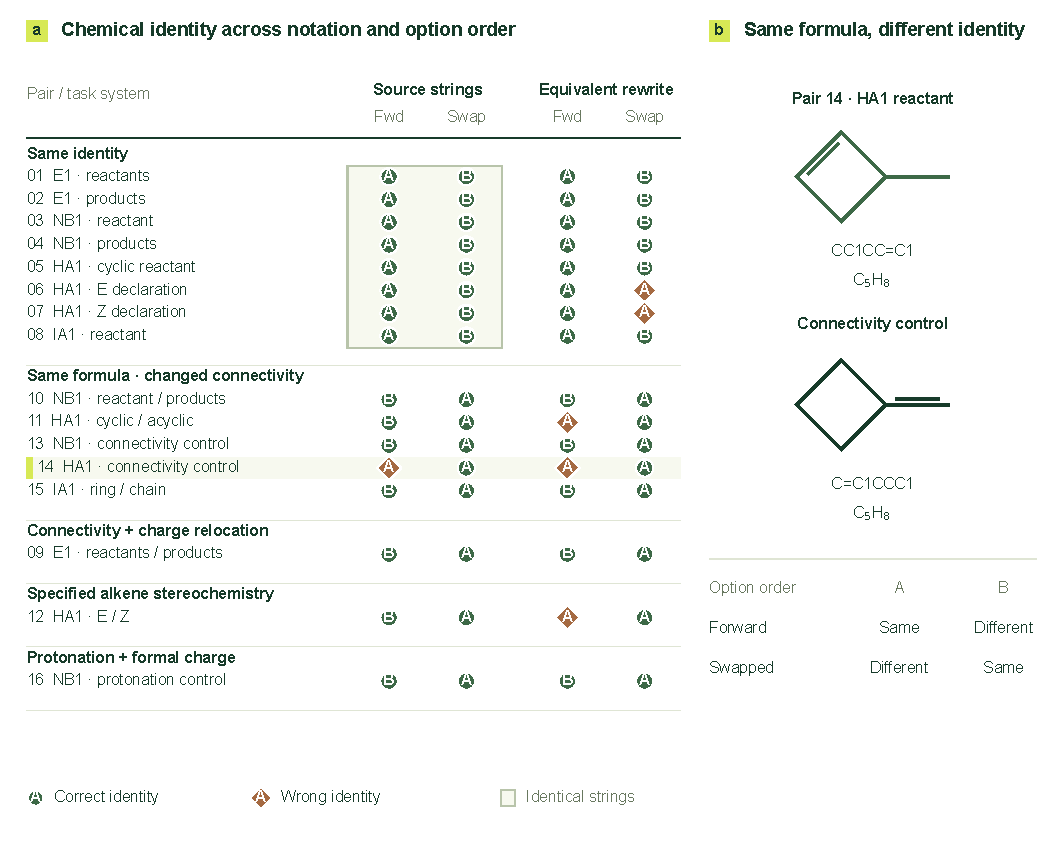
\includegraphics[width=\textwidth]{figures/fig06.pdf}
\caption{分子表示与选项顺序下的化学身份判断。16 对分子各包含四种输入条件；圆形和菱形分别表示正确与错误，内部字母保留模型实际回答。浅色区域为相同字符串条件。右侧显示第 14 对的两种 C\textsubscript{5}H\textsubscript{8} 连接结构及选项含义。 两种连接分别为 \texttt{CC1CC=C1} 与 \texttt{C=C1CCC1}，分子式均为 C\textsubscript{5}H\textsubscript{8}。}
\label{fig:06}
\end{minipage}
\end{figure*}

\begin{figure*}[!tbp]
\begin{minipage}{\textwidth}
\begin{minipage}[t]{.65\textwidth}
\vspace{0pt}
\centering
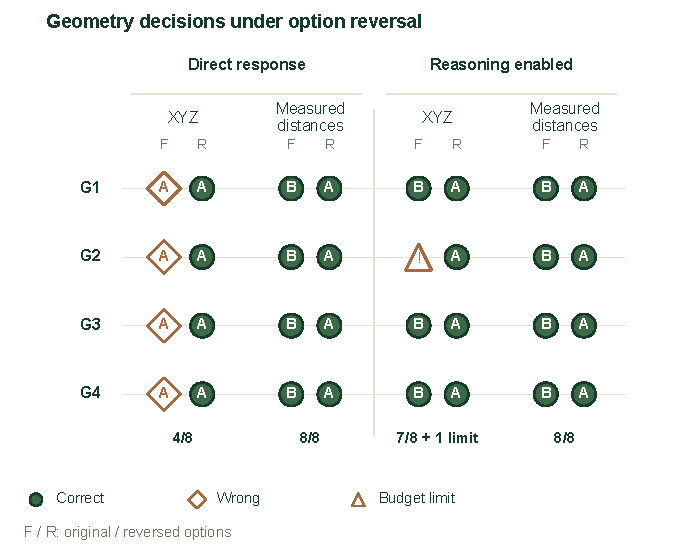
\includegraphics[width=\linewidth]{figures/fig07.pdf}
\caption{坐标输入与测量距离输入下的几何判断。四个源结构分别在直接回答和开启思考条件下比较，每种条件均包含原始（F）与交换（R）选项顺序。圆形表示正确，菱形表示错误，三角形表示达到输出预算；内部字母保留实际回答。}
\label{fig:07}
\end{minipage}\hfill
\begin{minipage}[t]{.31\textwidth}
\vspace{0pt}
\centering
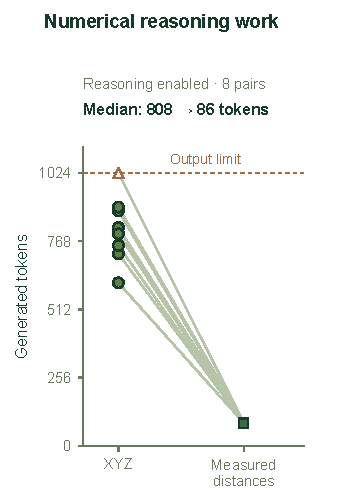
\includegraphics[width=\linewidth]{figures/fig08.pdf}
\caption{开启思考时的生成 token 数。每条线连接同一源结构、同一选项顺序下的笛卡尔坐标输入与测量距离输入，共八组配对比较。虚线表示输出上限。}
\label{fig:08}
\end{minipage}
\end{minipage}
\end{figure*}

\begin{figure*}[!tbp]
\begin{minipage}{\textwidth}
\centering
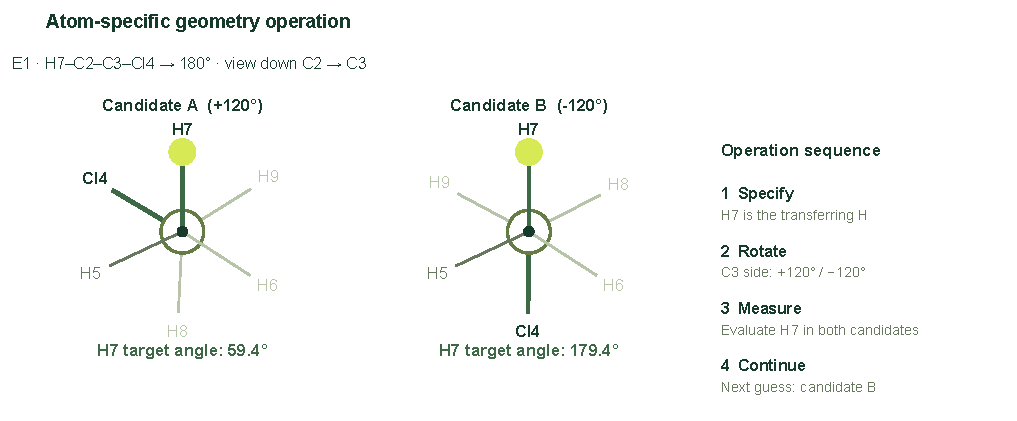
\includegraphics[width=.92\textwidth]{figures/fig09.pdf}
\caption{E1 中面向指定目标的几何操作。Newman 投影保留原候选坐标沿 C2\(\to\)C3 观察时的方向。H7 为指定的转移原子；候选 A、B 的目标角分别为 59.4° 和 179.4°。投影旁列出相应操作顺序。}
\label{fig:09}
\vspace{5pt}
\begin{minipage}[t]{.48\textwidth}
\vspace{0pt}
\centering
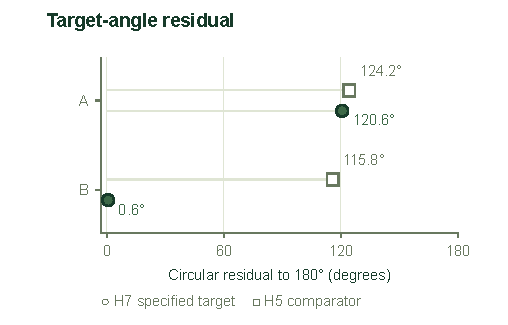
\includegraphics[width=\linewidth]{figures/fig10.pdf}
\caption{候选 A、B 相对指定 180° 目标的圆周角残差。H7 为指定目标原子，H5 为比较原子。}
\label{fig:10}
\end{minipage}\hfill
\begin{minipage}[t]{.48\textwidth}
\vspace{0pt}
\centering
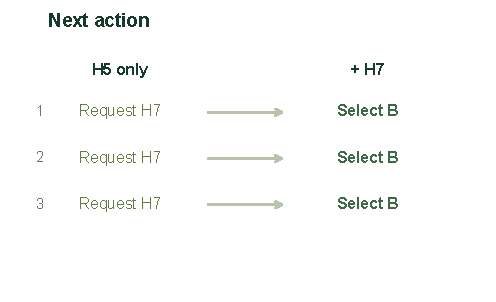
\includegraphics[width=\linewidth]{figures/fig11.pdf}
\caption{三种局部选项排列下的后续动作。仅提供 H5 测量值时，模型请求 H7 测量；补充 H7 后，模型选择候选 B。}
\label{fig:11}
\end{minipage}
\end{minipage}
\end{figure*}

\begin{figure*}[!tbp]
\begin{minipage}{\textwidth}
\centering
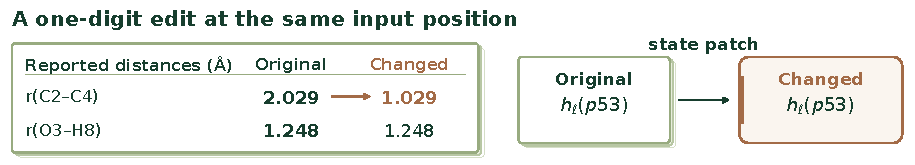
\includegraphics[width=.92\textwidth]{figures/fig12.pdf}
\caption{对单个报告距离的干预。一次数字修改将 C2–C4 距离从 2.029 改为 1.029 Å，O3–H8 保持 1.248 Å。在指定层，将原始输入中 token 位置 53 的残差状态替换到修改后输入的运行中。token 位置从零计数。}
\label{fig:12}
\vspace{4pt}
\centering
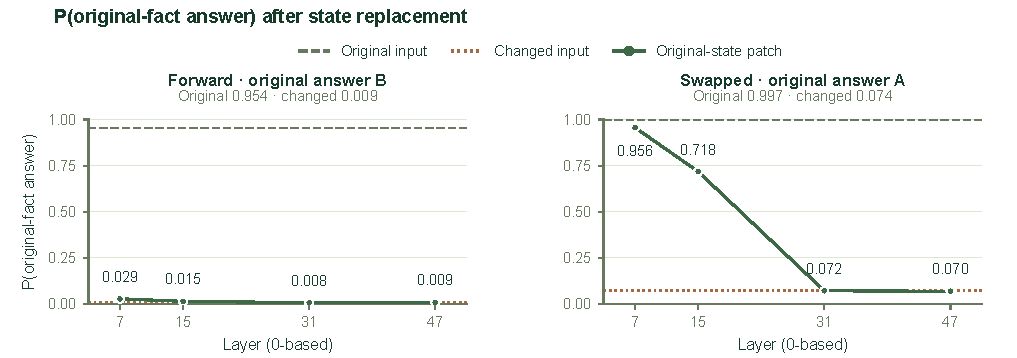
\includegraphics[width=.92\textwidth]{figures/fig13.pdf}
\caption{状态替换后原始事实答案的概率。曲线显示原始顺序（答案 B）与交换顺序（答案 A）下，原始事实答案在完整词表中的概率质量，包含无前导空格与带前导空格的 token 写法。水平线为原始输入与修改后输入的基线。层号从零计数。}
\label{fig:13}
\vspace{4pt}
\centering
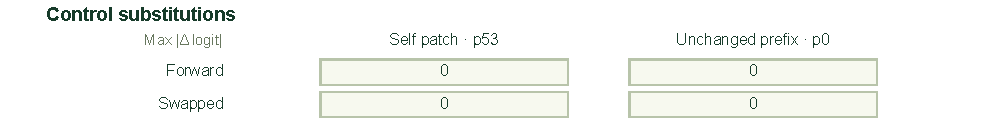
\includegraphics[width=.92\textwidth]{figures/fig14.pdf}
\caption{状态干预实验的对照替换。在 p53 进行同状态自替换，以及在 p0 替换未改变的前缀，两种选项顺序下均保持全部词表 logits 不变。表中报告 logit 差值绝对值的最大值。token 位置从零计数。}
\label{fig:14}
\end{minipage}
\end{figure*}

\begin{figure*}[!tbp]
\begin{minipage}{\textwidth}

\begin{minipage}[t]{.48\textwidth}
\vspace{0pt}
\centering
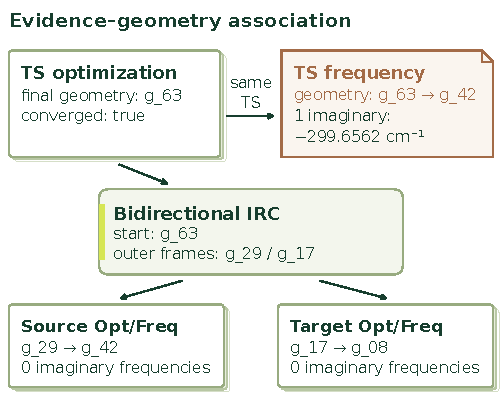
\includegraphics[width=\linewidth]{figures/fig15.pdf}
\caption{E1 源链中的证据与几何关联。受控输入将频率计算的几何引用从 g\_63 改为 g\_42，同时保持局部终止、收敛、能量和频率数值。图中保留从过渡态优化、双向 IRC 到端点优化与频率计算的关联。}
\label{fig:15}
\end{minipage}\hfill
\begin{minipage}[t]{.48\textwidth}
\vspace{0pt}
\centering
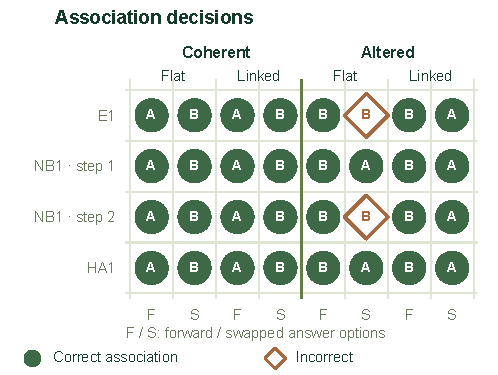
\includegraphics[width=\linewidth]{figures/fig16.pdf}
\caption{四条源链共 32 个输入的关联判断，交叉比较一致或修改后的关联、平铺或关联式表示，以及原始（F）或交换（S）答案顺序。字母保留已保存的 A/B 回答；圆形表示正确关联，菱形表示错误关联。}
\label{fig:16}
\end{minipage}
\end{minipage}
\end{figure*}

\begin{figure*}[!tbp]
\begin{minipage}{\textwidth}
\centering
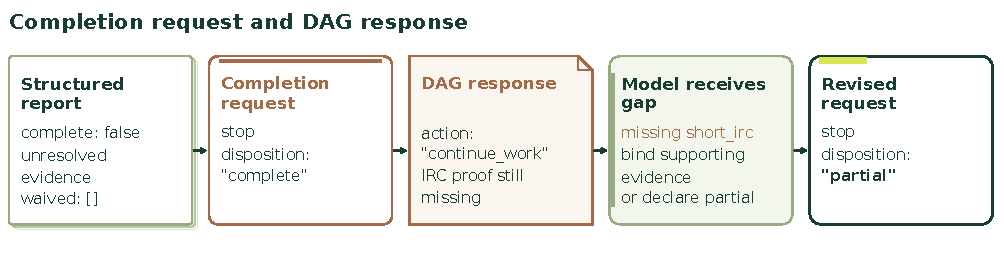
\includegraphics[width=.96\textwidth]{figures/fig17.pdf}
\caption{原始 IA1 轨迹中的完成请求与 DAG 反馈。报告仍有未解决的证据后，模型请求完成；系统指出缺少 short\_irc 证明并向模型反馈，随后模型改为请求部分完成。}
\label{fig:17}
\end{minipage}
\end{figure*}




















\subsection{端到端基准评估}

下文先报告最终整理后的综合分，再考察图结构、自洽性与准确度分量。离线整理从每次运行自身的研究材料组装机理图，并对齐已有评分记录，得到200次运行全部三项分量与综合分，整体均分为0.7051。图~\ref{fig:bench-overview}至图~\ref{fig:bench-tasks}据此区分最终交付、单项计算获得的科学支撑，以及结果与任务答案之间的对应关系。

\subsubsection{相对同一backbone，Cloudra提高了研究交付质量}

Guided 的综合均分为0.7803，Standard 为0.5940。50道题逐题配对的平均增益为0.1863，95\%任务 bootstrap 区间为[0.1003, 0.2759]。Guided 在35题中更高、8题中更低、7题持平，配对差值的中位数为0.1080（图~\ref{fig:bench-overview}）。差异因此出现在多个研究问题中，而非仅由最高分运行的少量提升形成。



各组最低分十题的均值也有差别：Guided 为0.3181，Standard 为0.0930。



最一致的改善出现在 Hard 立体化学任务。Guided 均分为0.9577，Standard 为0.6888，配对增益为0.2689 [0.1213, 0.4459]，十题中 Guided 全部更高。这些任务要求系统持续区分相互竞争的构型或通道，比较相应能垒，并将支持证据关联至对应结论。观察到的改善因此体现为一项比较性化学研究的完成质量，包括支撑立体化学判断的计算证据组织。

Normal 任务中，Guided 均分为0.7370，Standard 为0.5731，增益0.1640 [0.0365, 0.2922]，7题更高、3题更低。Easy 均分分别为0.8809和0.7305，但配对差值中位数为0.0209，其分布与 Hard 中广泛为正的改善不同。Impossible 均分分别为0.4451和0.2473；这组分数取决于运行是否回答了题目所要求的方法受限负结论，因而在后文单独分析。





\subsubsection{分量增益主要体现为计算证据的闭合}

拆开三项分数，可以定位工作流在哪一层出现差异（图~\ref{fig:bench-components}）。Graph 衡量交付物中所要求物种与步骤的覆盖及身份；Self-consistency 衡量鞍点、频率、IRC起点与端点优化/频率之间的支持关系；Accuracy 衡量结果与任务数值或负目标的符合程度。因此，一次运行可能给出接近参考的数值，而其路径证据仍未完整；也可能完成自洽的局部计算，却没有回答指定的研究问题。

全部50个 Guided--Standard 配对中，平均增益的加权图结构贡献为+0.0095，自洽性贡献为+0.1179，准确度贡献为+0.0589，合计对应综合增益0.1863。Normal与Hard的全部20题均差为0.2164，图结构、自洽性与准确度分别贡献+0.0080、+0.1247和+0.0837。



其中10道Normal题的三项贡献为+0.0098、+0.1141和+0.0400，10道Hard题为+0.0063、+0.1353和+0.1274。完整题库分解因此将收益同时定位到科学证据闭合与目标答案；Hard中准确度与自洽性的改善幅度相近。



HH1给出了直接例子。Guided 与 Standard 均交付联萘消旋能垒23.48 kcal/mol，接近参考23.01 kcal/mol；两者图结构均为1，准确度均约0.973。自洽性分别为1.0和0.5，对应综合分0.9838和0.8338。归档的 Standard 研究已有候选通道和 IRC 输入，但被接受的证据尚未形成所要求的端点连接；Guided 将路径证据关联至相应鞍点及端点。HI1呈现类似结果：两组准确度均约为1，自洽性由0.2333提高至1.0，综合分由0.7032提高至0.9999。这些对照定位到一个有价值的完成层次：得到有希望的数值答案之后，研究仍需把相关计算组织成可核对的证明。





\subsubsection{交付文件与分级科学支撑分别记录}

根目录交付图是否在运行中形成，与图中携带了多少科学证据，描述研究过程的不同部分（图~\ref{fig:bench-delivery}）。原运行中，Standard在50题中交付43份根图，Guided、Record与Brief-errors各交付50份。Standard未在运行中形成根图的7题为F1、HA1、HF1、IA9、M17、NR1和P3。离线整理从对应运行已有研究材料组装其机理图，最终各配置均形成完整50题记录。

Standard这7题整理后均分为0.1537，Guided在相同任务上的均分为0.8285，贡献了两组总净差的50.7\%；其逐题分数范围为0.0333至0.3425。这个对照将运行期结束判断与最终可交付的研究量联系起来：计算结果和候选描述可能已经留在运行记录中，而所要求的路径或比较结论尚未完成。整理后的机理图保留这一研究状态，并用于统一评价。



自洽分的分布进一步显示完整任务记录内部的差异。



各配置40道非Impossible任务中，Guided有24题的自洽连续分恰好为1、16题获得部分正分；Standard有7题满分、29题部分正分、4题零分；Record为16题满分、24题部分正分；Brief-errors各有20题满分与部分正分。图~\ref{fig:bench-delivery}并列展示完整证据分布与单独记录的运行期根图交付数，保留每项研究已建立的科学支持程度。

\subsubsection{消融区分能力可用与引导持续生效}

Record的全50题均分为0.7044，Brief-errors为0.7415。Guided相对Record高0.0759 [0.0121, 0.1438]，27题更高、8题更低、15题持平。Normal与Hard全部20题均差为0.1468，其中图结构贡献+0.0083、自洽性+0.0919、准确度+0.0466。保留工具及记录位置，与让未满足的科学要求在研究中持续参与后续动作选择，产生了不同结果。





\subsubsection{研究耗时与计算投入揭示不同的工作流收益}

图~\ref{fig:bench-speed}并列展示重复实验的耗时和 P2 可获得的计算投入。重复实验的测量单位是一个四题批次，批内并发度为2，每种配置实际观察3个批次。Guided、Standard、Record 和 Brief-errors 的平均批次耗时分别为4.451、3.958、3.894和4.827小时。Guided 平均比 Standard 长12.5\%，比 Brief-errors 短7.8\%。图中保留12个真实批次点及原始运行结果所对应的变异。这一测量包含批次的研究生命周期、计算等待及结果返回后的继续研究。

P2投入统计覆盖四组共有的15道深挖任务。Guided 每题使用11.08 job-hours，Standard 为7.55，Record 为7.88，Brief-errors 为15.59；对应最终综合均分分别为0.8124、0.6495、0.7360和0.7273。相对 Standard，Guided 累计计算时长多46.7\%，均分高0.1629；相对 Brief-errors，累计计算时长少28.9\%，均分高0.0851。在15个配对任务中，Guided 有7题同时比 Brief-errors 使用更少累计计算时长并得到更高分。



作业数量补充了这些投入的具体形式。共同任务中，Guided 记录789个量子化学作业，Standard 为419，Record 为431，Brief-errors 为883；其中失败作业分别为114、45、62和167，取消作业另行记录。NU3、NU5、NU6和NR1四道困难研究的16次运行共使用163.5 job-hours，占可用63条投入档案673.82 job-hours的24.3\%。相当一部分计算投入集中于这些追加尝试未能一致补齐网络缺口的研究。在归档的 Standard 缺图案例中，计算还可能晚于研究会话结束，使后续结果没有重新进入活跃研究。因此，结果返回后能否继续推进研究，也是这里所衡量的交付工作流的一部分。

Guided 相对 Brief-errors 的总体增益为0.0388，区间为[$-0.0317$, 0.1076]，26题更高、10题更低、14题持平。比较随研究要求改变：Guided 在 Normal 中平均高0.1514，在 Hard 中高0.1295，而 Brief-errors 的 Impossible 均分更高。结合共同任务的投入结果，这些观察支持进一步考察诊断究竟帮助系统修复什么：某个鞍点归属、路径端点、能量参照，或允许方法能否支持所要求的结论。更多诊断文字并未在所有这些决定上形成同一种排序。









\subsubsection{逐题差异定位需要持续维护的化学关系}

图~\ref{fig:bench-tasks}展示全部50题、四种配置及完整评分分量，既呈现稳定收益，也保留具体反例。Guided在Hard比较性研究中表现强，NB1和NI1也显示多步研究能够保持高分及充分证据。NB1中，Guided、Standard和Brief-errors分别为0.9628、0.9128和0.9900，Guided与Brief-errors的自洽性均为1；NI1中，Guided为0.9958，Standard为0.6196，自洽性分别为1和0.35。与此同时，NQ5中Record高于Guided，NU3中Brief-errors更高。这些差异使具体目标步骤与证据关系比按网络长度作单一排序更有解释力。

三个归档对照进一步说明哪些化学关系影响研究结论（图~\ref{fig:bench-cases}）。HA8中，Guided 给出29.46 kcal/mol，Standard 给出20.43 kcal/mol，参考为29.48 kcal/mol。档案将9.03 kcal/mol的差别追溯至能量参照：Guided 采用最低 all-s-trans 反应物极小值，Standard 采用反应性 cisoid 构象。



局部 IRC 连接和活化能所采用的稳定物种参照需要持续关联，同时分别记录：前者确定一条具体路径连接了哪些结构，后者确定研究问题要求的能量起点。



NU6显示路径身份也可能在计算后改变。Guided 记录的 concerted 鞍点能量为$-247.030042392$ Ha，betaine极小值为$-247.060060699$ Ha，两者差为18.836772 kcal/mol。Guided 将其描述为经过 concerted 鞍点区域的能量代价，并保留目标 betaine至产物闭环鞍点尚未找到的状态；Standard 则将18.837 kcal/mol交付为第二步闭环能垒。这个数值指纹将分歧定位到能差被解释为哪一个科学步骤。Guided 从 betaine 插值结构和受约束扫描峰出发的尝试，释放约束后反复回到直接反应物至产物的鞍点区域。因此，所要求的路径身份需要在优化后重新核对，不能直接从初猜名称继承。

这些例子与HH1的证据对照相互补充：同一个研究状态需要持续保留哪个构象定义能量参照、实际找到哪个驻点、它连接哪些端点，以及这些结果支撑哪个结论。Easy 逐题对照还区分了物理证据与参考匹配、结构化交付之间的差别。F4中，Guided 得分0.3601，Standard 为0.9083。Guided 交付了原生日志支持的16.016 kcal/mol氢负离子迁移能垒，分级自洽性为1；其准确度为0来自历史参考把反应物写为分离片段，而交付路径与参考能垒均针对Lewis加合物。

G2中，Guided 得分0.2389，Standard 为0.7769。Guided 原生日志支持约0.845 kcal/mol的双氢转移能垒。伴随边的数值能垒声明三次被拒绝后，Agent 删除了数值字段；Supervisor 反馈促使其恢复字段，但第四次拒绝及随后的鞍点证据检查后，最终图再次删除数值能垒以及鞍点能量、日志绑定。数值仅保留在文字说明中，准确度为0。Brief-errors 保留了相应数值结果，得分0.8500。

对 Guided 与 Record 的比较，F4与G2的综合分差分别为0.5566和0.5380，合计1.0946，占 Easy 总净劣势1.2679的86.3\%。D1、D3和L2中0.7的准确度来自既定数值偏差罚分上限。D1与 Standard 的能垒差追溯至反应物构象参照，D3则主要来自鞍点能量差。L2区分反应性cZc与更低的tZt参照；Standard 已交付相应的18.99与28.28 kcal/mol两种能垒，但参考匹配选中了前者。补充信息给出了这五题各工作流的分项得分、原生证据与事件顺序，全部正式分数保持不变。





\subsubsection{Impossible任务区分局部证据与目标负结论}

Impossible 组考察在 xTB/PM7 限制下能否得到题目规定的方法受限结论。Brief-errors 均分为0.4829，Guided 为0.4451，Standard 为0.2473，Record 为0.2325（图~\ref{fig:bench-imp}）。Brief-errors 相对 Guided 赢3题、负5题、平2题。其平均高0.0379，集中于特定答案：IA1贡献+0.8283，IA9贡献+0.5666；相反，IG8中 Guided 的结果在 Brief-errors减Guided方向贡献$-0.6661$。

IA1涉及环丁二烯方形几何的自同分异构目标，Brief-errors 的图结构、自洽性和准确度均为1，Guided 准确度为0。IA9涉及二氧杂环丁烷热分解，两组自洽性均为1，准确度分别为1和0。铬二聚体目标IG8则呈相反的准确度排序。在 Brief-errors 与 Guided 准确度相同的其余7题中，Brief-errors 平均低0.0500。



其 Impossible 总体优势分解为图结构$-0.0066$、自洽性$-0.0155$、准确度+0.0600：更高均分来自特定任务的目标结论，而 Guided 在另外一些任务中保留了更充分的局部支持。



全部40次 Impossible 运行中，4次准确度为1，14次同时具有自洽性1与准确度0。这一区别在分量矩阵中直接可见。例如，Guided 与 Brief-errors 在IA5、IC3和IF3中均得到自洽性1，却未获得目标负结论的准确度分；在兼含正负步骤的IB9中，两者准确度均为0.7。这些结果持续区分局部计算支撑与任务所要求的科学主张。

保存的 Brief-errors/IC3图提供了科学报告层面的具体例子。图中将最低开壳层单重态及相应状态转换边标记为不可达，拒绝给出所求单重态—三重态能隙；已经计算的闭壳层单重态仍作为独立表征分支保留，两个方法依赖的相对能量被明确排除在目标能隙之外。该运行保留了有效探索结果，同时没有把它们提升为关于另一个电子态的答案；其最终准确度分仍为0。这里同时保留科学声明与对应分数，状态映射问题放在讨论中处理。这个行为与IA1、IA9和IG8的得分逆转相互补充，明确指出了哪些结果可计算、哪些目标主张仍未获支持。


















\subsection{从化学意图到可靠空间操作}


后续小节利用归档研究轨迹及 Qwen3.8:27b 局部诊断，考察这些结果涉及的接口：化学身份、目标原子对应的几何操作、证据关联及结束研究的判断。原始轨迹定位具体研究问题；配对局部输入与内部状态干预则考察特定信息怎样改变判断和动作。

\subsubsection{化学身份为操作提供持续参照}



一次几何修改首先需要确定它作用于哪个分子、哪个原子和哪个反应中心。相同分子可以有不同的 SMILES 遍历方式；相同分子式也可以对应不同连接关系。为考察模型如何处理这些差别，我们构造了 16 对分子身份问题，覆盖相同身份、同分子式下的连接变化、连接与电荷位置变化、双键立体化学以及质子化变化。每一对交叉设置原字符串或等价改写，以及两种答案顺序，得到 64 次判断。



模型在其中 58 次作出正确判断。等价改写改变了 32 组表示配对中的 4 组语义判断，交换答案顺序改变了 32 组选项配对中的 6 组判断。后六组都重复选择字母 A。图~\ref{fig:06} 中的一对 C\textsubscript{5}H\textsubscript{8} 结构尤其直观：环内双键与环外双键对应不同连接方式，模型在四种条件下均回答 A，而 A 在两种顺序中分别代表“相同”与“不同”。这一结果将表示敏感性定位到实际的化学对象判断上，也说明持续研究需要保留稳定的身份参照。

Cloudra 的分子拓扑、原子映射与反应中心承担了这项职责。它们使模型在不同表述和不同构型间切换时，后续测量、片段移动及端点比较仍能指向原来声明的对象。原子对应关系还将产物端点对齐、路径插值与反应中心监测连接起来，使局部几何操作能够沿同一套化学身份继续进行。





\subsubsection{几何测量分担反复出现的数值推理}

识别研究对象之后，模型还需从坐标获得与操作有关的空间关系。我们选取 NB1 轨迹中的四个实际结构，要求比较两个指定原子间距。每个结构均交换答案顺序，并分别提供完整 XYZ 或程序测得的距离。两种信息条件进一步交叉直接作答与开启思考，形成 32 次原生聊天调用（图~\ref{fig:07}）。

直接作答时，XYZ 条件的八次响应全部选择 A，其中四次正确；提供测量距离后，八次均正确，并在选项交换后保持相同的语义答案。开启思考后，XYZ 条件得到七个正确答案，另一次在 1,024 个生成 token 时达到输出上限；该输入单独增加预算后，在 1,353 个生成 token 内得到正确答案。

测量距离条件的八次回答均正确。开启思考的八组配对中，XYZ 与测量距离条件的生成 token 中位数分别为 807.5 和 86。

这些结果提示，几何判断的负担包含原子定位、数值运算和关系比较。增加推理可以完成这些局部计算，程序测量则直接提供后续判断所需的关系量。Cloudra 因而让模型以键长、键角、二面角与片段关系表达目标，由确定性算子执行坐标变化。这种分工将重复的数值工作交给程序，并使操作后的变化能够直接检查，与程序辅助语言模型的职责划分相呼应。\citep{ref15} 分支拥挤描述、反应物预组织与局部片段旋转在此基础上，进一步把空间关系用于候选构型的选择和构建。





\subsubsection{反馈必须对应指定原子与几何目标}



确定性执行还需要与化学意图保持对应。E1 的一条真实轨迹提供了完整例子：模型希望将转移氢 H7、C2、C3 与离去原子 Cl4 调整为接近 180° 的二面角。它围绕 C2–C3 轴分别旋转 C3 一侧片段 +120° 与 \( - \)120°，构建候选 A 和 B，并将 C3–Cl4 距离调整到 2.35 Å。默认结构报告中的代表性二面角涉及 H5，而当前目标涉及 H7。模型随后主动计算两候选的 H7–C2–C3–Cl4，获得约 59.4° 和 179.4°，并在下一次实际提交中采用候选 B。

图~\ref{fig:09} 给出由保存的候选坐标绘制的 C2\(\to\)C3 方向 Newman 投影，图~\ref{fig:10} 汇总对应的目标角残差。

候选 B 的 H7 目标角距 180° 仅 0.6°，A 的相应残差为 120.6°；H5 比较量在两候选中的残差分别为 124.2° 和 115.8°。这组数据揭示了反馈的对象依赖性：一个读数的化学意义，来自它与当前指定原子及操作目的的对应关系。

围绕同一组测量值的局部对照进一步显示了信息与动作的连接。只提供 H5 时，三种循环选项排列均请求补测 H7；加入 H7 后，三种排列均选择 B。另两组充分性配对也随目标量的加入，从需要补测转为信息充分。由此，原子映射、内坐标、片段操作和反馈可以沿一条研究动作链理解：确定目标对象，执行空间改变，测量目标量，再选择下一候选。预组织、刚体对齐与路径准备也沿用这一对应关系，将反应意图传递到后续势能面探索。





\subsubsection{测量事实的内部传递影响选择}

局部对照可以单独考察一项几何事实怎样参与即时选择，并与研究轨迹中测量值经几何操作保留到后续判断的分析衔接。为进一步考察模型怎样使用已提供的测量值，我们在同一本地量化模型中进行了单位置激活替换。\citep{ref16} 输入中的一个距离由 2.029 Å 改为 1.029 Å，另一距离保持 1.248 Å，对应的比较答案随之反转。随后把原始输入在数字 token 位置的残差状态，分别替换到改动输入的第 7、15、31 和 47 层，并读取原始事实所对应答案的全词表概率。

替换的影响随层和选项顺序变化（图~\ref{fig:13}）。在交换选项的输入中，原始事实答案 A 的概率由改动后的 0.074，在第 7 和 15 层替换后分别升至 0.956 和 0.718；第 31 和 47 层的值分别为 0.072 和 0.070。在原选项顺序中，答案 B 的概率由 0.009，在前两层替换后分别变为 0.029 和 0.015，后两层仍接近改动输入。

自替换及未改变前缀位置的控制替换中，全词表 logit 差均为零。

替换一个数字位置的残差状态，改变了本探针中的后续选择。两种选项顺序下的差异与3.2.1节观察到的位置敏感性一致。结合测量与证据关联对照，这些结果支持将几何量与其化学对象和操作保持关联，使后续选择仍可对照同一组已记录事实。


\subsection{从局部计算结果到有证据的科学交付}


\subsubsection{DAG 保存结果之间的科学支持关系}

几何对象进入计算之后，研究需要把优化结构、能量、频率与路径逐步组织成对同一反应步骤的支持。每份结果的局部有效性及其归属共同决定这条支持链：频率应对应所声明的鞍点，IRC 应从该鞍点出发，两侧末帧的优化与频率应对应相应端点。DAG 将这些关系保存在物种与基元步骤上，为不断增加的结果提供持续的研究索引。执行状态、数值收敛与科学支持分别记录，使后续研究能够据此等待计算、调整重算或继续补充证据。

我们从归档提取四条源证据链，分别构造保持关联与改变单一引用的版本，并交叉平铺表示、关联表示和两种答案顺序，得到 32 个输入。单一引用的变化分别涉及频率几何、IRC 起始几何、端点优化输入或目标物种；局部终止、收敛、能量和频率值保持不变。图~\ref{fig:15} 以 E1 为例：将频率的几何引用从鞍点改为一个已有的端点，便改变了这份频率对当前步骤的支持关系。

关联表示的 16 次判断均正确，平铺表示的 16 次中有 14 次正确；两处错误均出现在引用已改变且选项交换的条件，分别来自 E1 与 NB1 第二步。随后选择的两条源链原生跟进中，开启思考使全部 16 次关联判断正确，包括原先两处错误。这一结果提示，明确关联可以分担模型查找与拼接计算关系的工作，也与图编码方式影响语言模型关系推理的观察相呼应。\citep{ref17} 在 Cloudra 中，这种表示进一步与真实计算产物绑定，使同一物种、步骤和尝试下的科学事实能够持续累积。

\subsubsection{诊断将缺口转化为具体研究动作}

诊断反馈把证据问题对应到需要修订的化学对象和计算。Cloudra 的结构化诊断指出具体问题，例如位阻冲突原子对、虚频模式对齐异常及路径端点连接问题，为下一次局部计算提供依据。

两条归档轨迹展示了这一过程。在 Brief-errors 的 HA1 试验中，简短错误代码替代了详细的 IRC 端点关联诊断。计算智能体反复更换源极小值引用，几何连接问题仍未解决。在 Guided 的 NB1 试验中，检查发现零虚频并返回模式诊断；协调智能体要求调整过渡态初猜参数和优化约束，计算智能体将这些改动用于下一次提交。这些案例说明诊断怎样把失败检查连接到需要处理的对象与参数。\citep{ref18}

各角色处理同一组已记录的化学实体。计算智能体优化分配步骤的几何和路径，协调智能体管理假设、分支与路线选择，Supervisor 对照任务要求审核累计支持。中央异步执行与持久化账本保留这些角色使用的计算记录和共享上下文。

\subsubsection{未完成项必须持续参与结束判断}

IA1 的归档轨迹中，一次结束请求与已记录的科学要求发生冲突。反应步骤仍缺必要的双向 short\_irc 验证，豁免清单为空。Supervisor 此前曾肯定中间体优化收敛，模型随后在 IRC 要求尚未满足时请求结束研究。

系统驳回该请求，并将尚缺的 short\_irc 要求返回模型。下一次提交中，模型将状态改为部分完成（图~\ref{fig:17}）。这项要求在局部计算获得肯定和之后的结束请求中持续保留。

我们还检验模型能否依据记录状态辨认 IA1 的未完成要求。在最新摘要与12条消息历史两种条件、正反选项顺序组成的6对输入中，12次判断均正确（100\%）。模型在每个状态问题及两种选项顺序下识别出未满足项。Delivery DAG 保留已确证对象与未完成要求，为继续计算或交付阶段性结果提供依据。

\subsection{工作流引导、科学判断与展望}

主对照表明，Cloudra通过使化学对象、计算结果与科学要求在探索中持续衔接，能够提高同一backbone的研究交付质量。Hard任务中一致的改善及Normal任务的收益，将这一贡献定位到比较性立体化学研究和多步研究的推进。完整50题分解显示，证据闭合与目标准确度均有收益；Hard中两项加权贡献分别为+0.1353和+0.1274。HH1和HI1进一步说明，即使已得到接近参考的能垒，数值结果与支撑其科学归属的路径证明仍是两个不同的研究成果。

归档案例提示，自主研究过程需要保持三种能力。首先，科学对象的身份需要超越当前语言描述而持续存在。一个反应物种可以包含多个构象，所要求步骤的初猜也可能优化至属于另一条路线的鞍点。HA8需要将能量分母持续关联至稳定物种，同时保留IRC实际连接的局部端点；NU6需要按优化后的连接关系判断新驻点，而非从初猜的预期名称继承身份。这些关系跨越了不同时间得到的计算结果。持续保存的研究图使模型能够在每次计算改变已知事实后，重新检查并更新这些关系。 这一解释与语言模型研究中外部规划、检验及反馈的作用相呼应。\citep{valmeekam2023planning}

其次，反馈需要指出研究应在哪一层改变。缺少端点优化与鞍点反复落到另一条路线需要不同动作，两者也不等同于方法无法描述目标电子态。语言模型依据当前上下文生成合理的后续动作；熟悉的化学表述可以保持连贯，而数值或路径证据已经发生变化。外部测量与结构化证据能够暴露这种失配，但智能体仍需判断应当修复计算、修改路径假设、重新选择参照，还是拒绝给出目标结论。Record对照说明，使工具可用并不足以保证这些关系持续进入最终论证；Brief-errors对照则说明，反馈中什么信息有用，取决于当前需要作出的决定；这一观察也呼应了外部反馈对推理修正作用的相关研究。\citep{ref18,huang2024selfcorrect} 文本解释对既有判断的合理化也为这种语义与证据脱节提供了相关研究背景。\citep{turpin2023unfaithful}

第三，完成局部证明与判断科学主张的范围需要共同推进。Brief-errors较高的Impossible均分来自IA1和IA9的特定目标结论，IG8则呈相反结果。其IC3图提供了更具体的行为证据：运行保留已表征的闭壳层分支，同时拒绝将其当作所求最低开壳层单重态，或把其相对能量报告为目标能隙。这是一种有价值的科学判断：保留探索已经建立的结果，同时不让方便得到的结果替换原本不同的研究问题。交叉结果支持一个依赖任务的解释假说：详细诊断有助于补齐有效的局部证明，但当方法或目标本身需要重新审视时，持续修补当前证明可能无助于解决问题。本次最终结果对照并未确立诊断长度的因果作用，也未测量其背后的模型内部认知机制。

Easy反例中的失分有两种不同来源。F4的冻结参考将以Lewis加合物为起点的能垒关联至分离片段，这是参考目标身份的问题，并非对其已检验路径的否决。G2则暴露了工作流之间的相互作用：伴随边通过检查前阻止数值声明，促使智能体删除了原生计算已经支持的数值；Supervisor反馈曾恢复这些字段，后续拒绝又先于最终删除。这里需要区分保存暂定观测与接受该观测所支撑的机理主张。验收状态应限定归档数值的科学用途，同时保留数值及来源。两条轨迹并不支持将Easy组失分统一归于低频虚频或IRC收敛拒绝，其保留的自洽分量也不符合完整性短路归零规则。

分数与主张记录还显示了评价器需要进一步区分的科学身份。Record/IA5正确拒绝目标异旋路径，但归档裁定记录了匹配器选择另一条相同端点正路径的情况；Brief-errors/IC3尽管明确区分目标开壳层态及独立闭壳层分支，准确度仍为0。本文保留定稿分数，并与保存的科学主张一同解释。这些案例说明，仅有分子连接关系不足以标识反应通道或电子态目标；评价过程也需要保留研究工作流旨在维持的状态与路径区别。

SI按原有负目标计分规则，对IA5与IC3的所求对象开展条件性匹配分析，固定两例的图分、自洽分及其余198次运行。每次对象归属修正使一例综合分由0.4变为1.0，对应配置的Impossible均分增加0.0600。两项同时修正时，Brief、Guided、Record和Standard的条件均分分别为0.54294、0.44506、0.29250和0.24733。Brief、Guided、Record之间的排序不变，Record超过Standard；Guided与Standard的每一对比较均不变。正式分数和图仍保留原值，条件分析表将对象匹配与智能体最终科学判断分别呈现。

P2每题每配置保留一次运行，任务簇bootstrap区间反映抽样题目构成的变化，不刻画同一任务独立重复运行的随机方差。另行开展的P1b研究在四题、四配置的每个组合上重复三次，共48次运行，并未为P2的全部50题提供重复测量。完整整理后的P2表覆盖200次运行及其三项评分分量。部分Hard任务的准确度目标是定性通道身份，因此收益包括路径识别、证据闭合和数值能垒。后续对完整题库重复评估，可以进一步刻画运行间变异及不同研究路线的选择频率。

Impossible组按允许方法契约定义，不是对相应化学普遍不可能发生的断言。其分量还采用负目标规则，显式负结论的自洽性1与正路径的TS—IRC—端点证明分别解释。14例自洽性1、准确度0因而需要结合目标主张与来源理解。NU6能量指纹吻合则定位到可达路径中的相关问题：当鞍点身份与所要求步骤没有持续关联时，同一个能差可能被赋予不同科学含义。这些案例支持在研究假设改变时，持续检查每次计算实际回答了什么。

耗时与投入同样按实际观测单位报告。12个先导批次测量并发度2的四题真实耗时，包含原始失败与停止结果；P2投入档案覆盖选定的深挖研究，四配置共有15题。累计job-hours代表记录的量子化学进程时长，Standard/M1另有已注明的原生日志重构；它与核时、费用及P2端到端研究耗时分别记录。并发计算共享资源，CPU排队可能延迟个别结果。因此，这些测量支持已观察工作流与投入之间的比较；进一步区分排队、计算及智能体活跃时间，有助于明确实际耗时花在何处。

交付案例还给出了与科学改进相对应的系统方向。等待计算、收到完成事件、恢复研究及形成最终产物，需要共享连续的任务生命周期。Standard的缺图源于计算尚未完成时的提前结束；Guided/HI1也暴露了通知没有唤醒等待会话的问题。使未完成目标持续跨越这些状态变化，才能把新完成计算变成可用的研究信息。科学层面还需要让反复返回同一驻点区域的现象保持可见，帮助智能体判断再做一次局部尝试是否足以解决目标路径。更好的候选选择及研究假设修订，可以进一步补充证据保存能力的改善。

Cloudra的默认预组织采样32个刚体相对放置，进行局部MMFF94松弛，再按能量与聚类选择候选。这一流程采样局部排布。频率确证的极小值表明驻点性质合格，不能据此判断所有更低构象均已搜索。HA8说明需要同时保留规定的稳定参照与局部活性构象，而全局最低点的主张还需要单独评估构象覆盖。CREST通过独立的可选后端提供，本次200次运行并未建立统一的CREST覆盖。高柔性体系可能需要更广的构象采样与更多量子化学计算。后续需要测量构象覆盖程度，并改进相互竞争候选之间的计算资源分配。

本基准比较纯电子能差，未加入零点能、热与熵、标准态校正，也未量化溶剂化对自由能的贡献。NI5的题设为弱酸性水溶液，NU5则为高浓度二氯甲烷条件，这一区别对二者尤为重要。其分数评价规定的电子能参照。对于缔合与解离，熵及浓度相关的标准态项进入$\Delta G^\ddagger$；溶剂参与还可能改变描述路径所需的化学模型。推断溶液条件下的控速步骤或立体选择性，需要对相关物种和路径采用一致的自由能处理。本研究未开展溶剂敏感性对照，因此不据此推断实际溶剂影响的大小或方向。

原子映射系数与歧义窗口，以及分支拥挤描述符的衰减、深度和拥挤设置，在各工作流对照中保持固定。本研究未通过参数扫描测量各项设置的敏感性或独立贡献。虚频模式对齐比值0.5仅用于提示，科学验收由驻点与IRC端点证据决定。P2各配置均使用DeepSeek-v4.1-flash（1017），归档API别名为\texttt{deepseek-v4-flash}，请求设置另行保留。采用更多backbone进行比较，可以检验工作流收益在不同模型间的适用范围。

我们的长期目标是将Cloudra从小分子机理计算扩展至更广泛的计算化学领域。多种计算引擎支持、共享执行基础设施及持续保存的科学记录，已为这一扩展提供基础；面向新的问题类型，还需要相应的科学表示、计算方法与验证准则。我们希望Cloudra最终成为计算化学家的强大研究工具，以及实验团队的计算专家。Cloudra将以GNU Affero General Public License（AGPL）开源，支持系统的公开检查、复用与社区共同发展。

